\subsection{Verifica}
\subsubsection{Scopo}
Il processo di verifica ha come obiettivo la realizzazione di prodotti corretti, completi e coesi secondo delle norme stabilite. Sia il software che la documentazione devono essere sottoposti al  al processo di verifica.

\subsubsection{Descrizione}
Con la verifica si cercano e  risolvono i possibili difetti presenti all'interno della documentazione e del codice. Essa viene applicata ad ogni altro processo in esecuzione quando questo:
\begin{enumerate}
    \item Raggiunge un livello di maturità sufficiente;
    \item Subisce dei cambiamenti significativi.
\end{enumerate}
Dopo che la verifica è ultimata è possibile avviare il processo di validazione.

\subsubsection{Aspettative}
L'input del processo di verifica è un processo già ben formato ma non necessariamente corretto; l'output è il processo stesso reso conforme alle aspettative. Questo risultato si ottiene seguendo determinati punti:
\begin{enumerate}
    \item Definizione di un criterio di accettazione;
    \item Definizione delle attività di verifica;
    \item Definizione e implementazione di test di verifica;
    \item Correzione di eventuali difetti individuati.
\end{enumerate}

\subsubsection{Verifica della documentazione}
L'inizio delle attività di verifica per un documento è stabilito dal \textit{Responsabile di Progetto} che ne pianifica le date di inizio e di fine e assegna il ruolo di \textit{Verificatore} ad uno o più membri del gruppo. I verificatori dovranno eseguire un'analisi accurata del documento assegnatogli con l'obiettivo di:
\begin{enumerate}
    \item Verificare la correttezza grammaticale e la semplicità sintattica;
    \item Assicurarsi che il documento rispetti tutte le norme tipografiche descritte accuratamente in \ref{_normetipografiche};
    \item Controllare la struttura del documento;
    \item Analizzare la pertinenza dei contenuti trattati nel documento.
\end{enumerate}

\paragraph{Analisi statica}
Questo tipo di analisi viene effettuata sul prodotto senza eseguirlo e serve per verificare che non ci siano errori. I due tipi di analisi statica sono:
\begin{itemize}
    \item \textbf{Walkthrough}: consiste nell'analizzare il documento nella sua interezza per trovare i difetti. Viene usata principalmente nella prima fase di verifica;
    \item \textbf{Inspection}: tecnica che prevede la focalizzazione sui punti in cui si sa che si concentrano gli errori. Questo metodo è da preferire rispetto a \textit{walkthrough} poiché molto meno oneroso. Tuttavia si può utilizzarlo solo dopo una fase di verifica iniziale a pettine (di tipo \textit{walktrough}) che permette di acquisire una lista di errori comuni denominata \textit{Lista di Controllo}.
\end{itemize}

\paragraph{Procedimento di verifica della documentazione}
\begin{figure}[h!]
    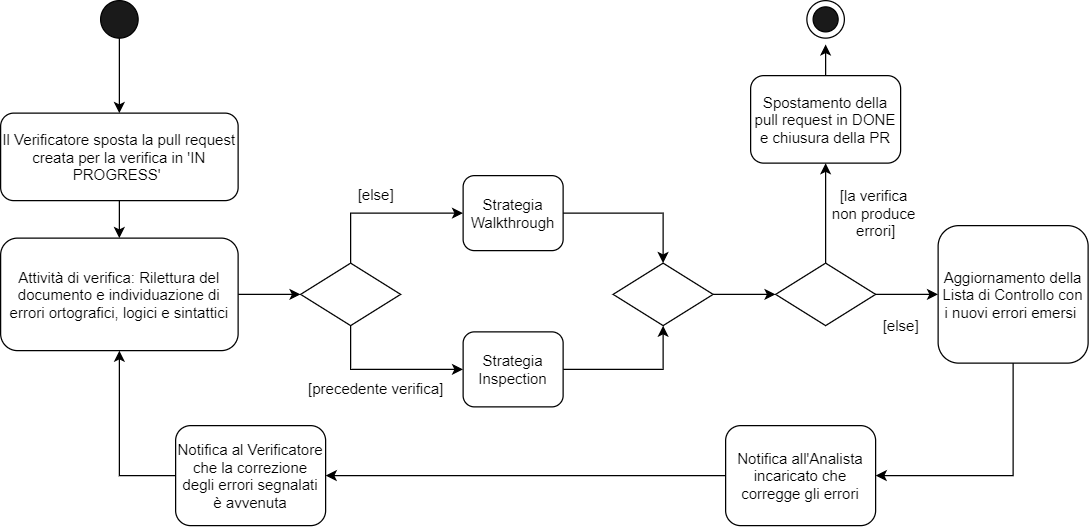
\includegraphics[width=\linewidth]{res/images/processo_verifica.png}
    \caption{Processo di verifica  dei documenti}
\end{figure}
Il processo di verifica viene gestito con il meccanismo delle pull request, una sorta di issue avanzata messa a disposizione da \glock{Github} descritto in dettaglio in \ref{_cicloVitaAttivita}.

\subsubsection{Verifica del codice}
Il codice viene verificato con test automatici e con misurazioni quantificabili specificate all'interno del \dext{Piano di qualifica}. Il codice quindi deve obbedire a questi criteri:
\begin{itemize}
    \item Deve essere corretto rispetto ai test definiti e alle metriche adottate per quantificare la sua qualità;
    \item Deve derivare dai requisiti richiesti in \dext{analisi dei requisiti}.
\end{itemize}

\paragraph{Analisi statica}
Anche per il codice, come per la documentazione, la prima fase di verifica sarà caratterizzata dall'analisi statica. %per gli strumenti si aspetta di iniziare a fare codice

\paragraph{Analisi dinamica}
L'analisi dinamica prevede la verifica del codice mirata a rilevare gli errori mentre questo è in fase di esecuzione.  Questa fase è caratterizzata dall'esecuzione di una batteria di test per verificare il corretto funzionamento del codice prodotto.\\
Ogni test eseguito deve essere:
\begin{itemize}
    \item \textbf{Decidibile}: sempre in grado di terminare restituendo un feedback binario (riuscito/ fallito);
    \item \textbf{Ripetibile}: dato un certo input e delle precondizioni fissate, deve produrre sempre lo stesso output per ogni prova effettuata.
\end{itemize}
Ogni test presenta i seguenti parametri:
\begin{itemize}
    \item \textbf{Ambiente}: caratteristiche hardware e software sulle quali viene eseguito il test;
    \item \textbf{Stato iniziale}: lo stato del software al momento dell'avvio del test;
    \item \textbf{Input}: dati in ingresso inseriti;
    \item \textbf{Output}: dati in uscita attesi;
    \item \textbf{Ulteriori istruzioni}: ulteriori informazioni sulla configurazione iniziale, sull'interpretazione dei risultati ottenuti e sugli eventuali effetti collaterali che l'esecuzione può produrre.
\end{itemize}
Per il formato di output di un test è da preferirsi un file di log che esponga in maniera chiara e immediata i risultati.

\subsubsection{Verifica dei requisiti}
Anche i requisiti sono sottoposti al processo di verifica. Perché la verifica dia esito positivo è necessario che essi:

\begin{itemize}
    \item Siano coerenti con la loro implementazione;
    \item Abbiano un grado di complessità adeguato rispetto al tempo e alle risorse pianificate per la riuscita del progetto;
    \item Si dimostrino verificabili e quantificabili;
    \item Siano coerenti con gli accordi presi con il proponente, riportati all'interno dell'\dext{analisi dei Requisiti}.
\end{itemize}

\paragraph{Analisi statica}
I requisiti devono rispettare le proprietà di:
\begin{itemize}
    \item \textbf{Verificabilità}: un requisito deve essere misurabile oggettivamente;
    \item \textbf{Codice univoco}: un requisito deve essere identificato da un codice, differente per ogni requisito, in accordo con quanto descritto in \ref{_classificazioneRequisiti};
    \item \textbf{Atomicità}: un requisito non deve essere divisibile.
\end{itemize}

% \subsubsection{Test}
% I test costituiscono l'attività fondamentale dell'analisi dinamica: permettono di individuare i bug e di dimostrare che l'applicativo sviluppato è conforme rispetto a tutti i requisiti concordati nell'\dext{analisi dei requisiti}.\\
% Verranno implementati tipi di test descritti di seguito, ognuno con uno scopo diverso e con un oggetto di verifica differente.
% \paragraph{Test di unità}
% Consiste nel testare la partizione più piccola di software: l'unità. Il corretto funzionamento di ogni unità deve essere testato prima di procedere alla sua integrazione.

% \paragraph{Test di integrazione}
% Necessari per testare che le diverse unità si interfaccino correttamente: questo tipo di test è eseguito in maniera ricorsiva: ogni volta che un gruppo di unità esegue in maniera corretta questo viene testato unendolo ad un altro gruppo di unità via via più grande fino ad arrivare al test di sistema.

% \paragraph{Test di sistema}
% Dopo che tutte le unità sono state testate ed è stata testata la loro integrazione viene eseguito il test dell'intero sistema. In questa fase si verifica che tutte le componenti interagiscano nel modo atteso e che l'applicazione soddisfi ciò che è stato definito nell'\dext{analisi dei requisiti}.

% \paragraph{Test di regressione}
% Quando una o più unità vengono modificate si esegue questa tipologia di test che serve per accertarsi che le funzionalità precedentemente implementate e testate non siano state danneggiate dai cambiamenti apportati al software.

% \subsubsection{Procedimento di verifica del codice}
% \subsubsection{Strumenti}